\documentclass{anstrans}
%%%%%%%%%%%%%%%%%%%%%%%%%%%%%%%%%%%
\title{Evaluation of anisotropic interfacial properties of $\alpha$-U via molecular dynamics}
\author{Khadija Mahbuba,$^{1}$,Benjamin W. Beeler,$^{1}$^,$^{2}$ Andrea Jokisaari,$^{2}$ }

\institute{
$^{1}$North Carolina State University, Department of Nuclear Engineering, Raleigh, NC 27607
\and
$^{2}$Fuel Modeling and Simulation Department, Idaho National Laboratory, Idaho Falls, ID 83415

}

%%%% packages and definitions (optional)
\usepackage{graphicx} % allows inclusion of graphics
\usepackage{booktabs} % nice rules (thick lines) for tables
\usepackage{microtype} % improves typography for PDF
\usepackage{verbatim} 
\usepackage{placeins} 
\usepackage{gensymb}

\newcommand{\SN}{S$_N$}
\renewcommand{\vec}[1]{\bm{#1}} %vector is bold italic
\newcommand{\vd}{\bm{\cdot}} % slightly bold vector dot
\newcommand{\grad}{\vec{\nabla}} % gradient
\newcommand{\ud}{\mathop{}\!\mathrm{d}} % upright derivative symbol

\begin{document}
%%%%%%%%%%%%%%%%%%%%%%%%%%%%%%%%%%%%%%%%%%%%%%%%%%%%%%%%%%%%%%%%%%%%%%%%%%%%%%%%
\section{Introduction}
Two life-limiting phenomena in metallic fuels are fission gas release and fuel-clad chemical interaction (FCCI) \cite{carmack2009}, both of which are affected by fuel swelling driven by the development of porosity and fission gas bubbles. Fuel swelling in U-Zr metallic fuel is anisotropic and highly dependent upon the phase of U \cite{hofman2015}. Within metallic fuel, it is expected that all three U allotropes are present due to both the temperature gradient across the fuel slug and the alloying composition. The low-temperature allotrope of U, $\alpha$-U, is stable up to 935 K \cite{hofman1996} and has a low symmetry orthorhombic structure with four atoms in the unit cell. Polycrystalline $\alpha$-U displays complex behavior due to the fundamental anisotropy of the crystal structure and the presence of internal microstructure \cite{barrett2020}. Because grain boundaries (GBs) act as sinks for irradiation-induced point defects and also hinder dislocation movement, they are a very important feature affecting the deformation and plasticity of $\alpha$-U.

The ability to predict the microstructural evolution of $\alpha$-U under irradiation and subjected to temperature gradients relies on an accurate understanding of interfacial properties, including GB and surface energies. Such energetic properties can serve to provide fundamental insight into the expected fission gas bubble behavior, interfacial orientations, GB mobility, and tearing. The current work performs a computational analysis to evaluate the GB energy and surface energy related to STGBs by molecular dynamics. Interfacial energies are determined as a function of misorientation angle. Using grain boundary energies and corresponding surface energies, the work of adhesion for different STGBs is evaluated. The interaction of point defects with grain boundaries is examined to establish both an interaction distance and a grain boundary bias.


%%%%%%%%%%%%%%%%%%%%%%%%%%%%%%%%%%%%%%%%%%%%%%%%%%%%%%%%%%%%%%%%%%%%%%%%%%%%%%%%
\section{Computational Details}

The Large-scale Atomic/Molecular Massively Parallel Simulator (LAMMPS) \cite{plimpton1995} is utilized to perform molecular dynamics (MD) simulations. A simulation box is selected and divided into two regions to generate the supercell. Region one is tilted by \textit{$\theta$/2}, without distorting the lattice of $\alpha$-U, with respect to the defined tilt axis, where \textit{$\theta$} is the misorientation angle and the tilt axis is parallel to the tilt plane (or cut plane). Taking the reflection of the former region across the tilt plane, region two is created, and, in the process, two symmetric tilt GBs are generated; one in the center of the supercell, and one across the periodic boundary normal to the tilt plane. To generate the surface, region two (or the mirrored region) of the supercell is considered a vacuum. 

The size of the supercell depends on the orientation of the STGB plane or surface investigated, which is selected such that the two-grain boundary planes or surfaces present within a single supercell are non-interacting while also satisfying periodic boundary conditions in all directions. Thus, the number of atoms varies by grain boundary geometry, ranging from 968 to 4,800 atoms. System sizes were observed to be converged with respect to interfacial energy. In this work, we utilize a STGB nomenclature of (\textit{h k l})$\langle$p q r$\rangle$, where (\textit{h k l}) is the misorientation plane and $\langle$p q r$\rangle$ is the tilt axis. A total of twenty-four STGBs with tilt axis $\langle$1 0 0$\rangle$ and shear plane (0 0 1) were generated. These grain boundaries (or surfaces) of (\textit{h k 0})$\langle$1 0 0$\rangle$ are further referred to as type A grain boundaries \cite{mahbuba2021}.

The UMo angular dependent potential (ADP) from Starikov \cite{starikov2018} is used in this work. This interatomic potential reasonably predicts a number of properties in $\alpha$-U, $\gamma$-U, and $\gamma$-UMo alloys. A Nose-Hoover barostat is considered for the anisotropic relaxation of the system in all directions with a damping factor of 0.1. For temperature control, a Langevin thermostat is utilized with a relaxation time of 0.1 ps. The system is observed at 500 K, where U is present in the $\alpha$ phase. When the volume and energy of the system reach equilibrium, the values of observable parameters (energy and volume) are collected. Systems are equilibrated for 200 to 250 ps, and energies are averaged over the final 50 ps. To ensure statistical significance, each system is simulated three to five times, each with a unique initial distribution of velocities. This yields a maximum standard error of approximately 5\% for interfacial energies.

The interfacial energies are calculated as
%
\begin{equation}
\label{eq:eform}
E_{\mathrm{inf}} = \frac{E^*-E_0}{2A} \times N
\end{equation}
%
where $E_{\mathrm{inf}}$ is the interfacial (STGB or surface) energy per unit interface (STGB or surface) area, $E^{*}$ is the internal energy per atom of a system with an interface, \textit{N} is the number of atoms in the system with an interface, $E_{0}$ is the internal energy per atom of a defect-free system, and \textit{A} is the area of each interface (as there are two interfaces per supercell, there is 2\textit{A} in the denominator). In addition, the work of adhesion of STGBs is calculated as
%
\begin{equation}
\label{eq:fform}
W_{\mathrm{ad}} = 2 \times E_{\mathrm{inf(surface)}}-E_{\mathrm{inf(STGB)}}
\end{equation}
%
where $E_{\mathrm{inf(surface)}}$ is the surface energy per unit area and $E_{\mathrm{inf(STGB)}}$ is the GB energy per unit area.

To determine the defect interaction with a grain boundary, a single defect (either vacancy or interstitial) is inserted a prescribed distance from the grain boundary. The formation energy of a defect is determined from equation \ref{eq:3}

\begin{equation}
\label{eq:3}
E_f = E^d - \frac{N\pm1}{N}\times E^p 
\end{equation}

where E$^d$ is the total energy of a system with a defect and two grain boundaries, E$^p$ is the total energy of a pristine system with no defects (however this system does include two grain boundaries) and \textit{N} is the total number of atoms in the pristine reference system. Ten unique simulations are performed to gain statistical significance of the results.

%%%%%%%%%%%%%%%%%%%%%%%%%%%%%%%%%%%%%%%%%%%%%%%%%%%%%%%%%%%%%%%%%%%%%%%%%%%%%%%%
\section{Results and Analysis}

\subsection{Grain Boundary Energies}

The GB energy calculated for all twenty-four STGBs is plotted as a function of misorientation angle in Figure~\ref{fig:1} at 500 K. Deep cusps are observed at the (0 1 0) and ($\overline{3}$ 12 0) plane, with corresponding GB energies of 0.36 J/m${^2}$ and 0.27 J/m${^2}$. At 0$\degree$ and 360$\degree$, both regions (tilted and mirror of tilted) of the supercell have their major axis ($\langle$1 0 0$\rangle$ and $\langle$0 1 0$\rangle$) parallel to their respective axes of the supercell. As $\alpha$-U does not have mirror symmetry with respect to the (0 1 0) plane, a GB is created at the junction of two regions, albeit with a small atomic misfit. Thus, the (0 1 0) and (0 $\overline{1}$ 0) orientations have a cusp in the GB energy profile. At the 180$\degree$ misorientation, both regions have their $\langle$0 1 0$\rangle$ axis parallel to the $\langle$1 0 0$\rangle$ axis of the supercell. Because of the symmetry of the (1 0 0) plane of $\alpha$-U, this orientation does not describe any GB and is instead the pure crystalline system, resulting in zero grain boundary energy. As seen in Figure~\ref{fig:1}, the highest GB energy is 0.9 J/m${^2}$, which occurs at the 14.25$\degree$ misoriented STGB ($\overline{12}$ 3 0)$\langle$1 0 0$\rangle$. The GB energy increases as the misorientation increases up to 15$\degree$, and decreases as misorientation increases to 180$\degree$ (neglecting the cusp). The shape of the GB energy versus misorientation angle has a mirror symmetry with respect to the (1 0 0) plane. This set of STGBs has an average grain boundary energy of 0.71 J/m${^2}$, as obtained by simple averaging. Because the lowest GB energy is the ($\overline{3}$ 12 0)$\langle$1 0 0$\rangle$ orientation, it would be a likely candidate to form twins. Without considering the major cusps (very low energy STGBs), the average GB energy of general STGBs is 0.78 J/m${^2}$. It has been experimentally observed that $\alpha$-U grains are always oriented in a direction that is more than 60$\degree$ from the $\langle$1 0 0$\rangle$ direction (i.e. around the $\langle$0 1 0$\rangle$ direction) \cite{stobo1965}. We show that STGBs tilted with respect to the $\langle$1 0 0$\rangle$ axis between 63.4$\degree$ to 116.6$\degree$ have very low energies (0.23 J/m${^2}$ to 0.72 J/m${^2}$, which is equal or lower than the average GB energy. This seems to support the previous experimental findings. 

\begin{figure}[ht] % replace 't' with 'b' to force it to be on the bottom
  \centering
  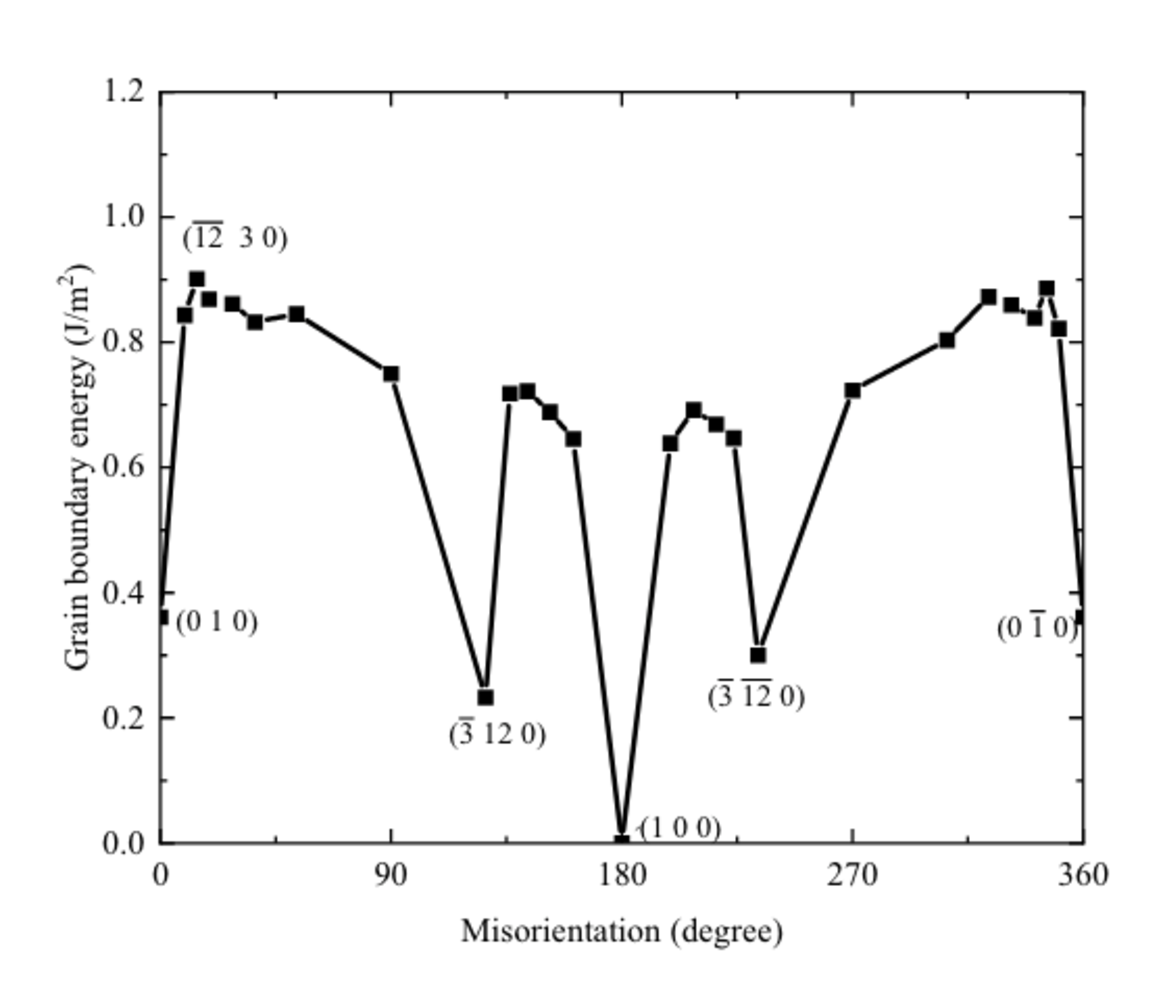
\includegraphics[width=\columnwidth]{fig1}
  \caption{The Grain Boundary Energy as a function of misorientation angle at 500 K.}
  \label{fig:1}
\end{figure}

As no data on GB energies in $\alpha$-U are available for comparison, the current computational work is compared with previous computational studies of $\gamma$-U. The high-temperature $\gamma$ phase of U has a body-centered crystal structure. $\gamma$-U \cite{beeler2018} was found to have a GB energy from 0.3 J/m${^2}$ - 0.45 J/m${^2}$, whereas $\alpha$-U STGBs possess a GB energy from 0.23 J/m${^2}$ - 0.91 J/m${^2}$. Thus, there are good quantitative comparisons for GB energies amount these two systems, although the magnitude of non-cusp $\alpha$-U grain boundaries is generally higher than those of the $\gamma$ phase.

\subsection{Surface Energies}

The surfaces considered in this work are only those which are related to the STGBs. For instance, a STGB characterized by ($\overline{3}$ 6 0)$\langle$1 0 0$\rangle$ will be analyzed as a surface characterized by ($\overline{3}$ 6 0). The effect of tilt angle (surface orientation) on the surface energy is plotted in Figure~\ref{fig:2}. The surface energies of the (1 0 0) and (0 1 0) planes have also been evaluated. The tilt angle of the studied surfaces ranges from 0$\degree$ to 180$\degree$ and the energies are characterized at 500 K. Data points are connected by straight lines to guide the eye.

The average surface energy is found to be 1.25 J/m${^2}$, with the minimum energy surface observed for the ($\overline{3}$ 12 0) (symmetric $\overline{3}$ $\overline{12}$ 0)) plane, at 1.0 J/m$^2$. Interestingly, the ($\overline{3}$ 12 0)$\langle$1 0 0$\rangle$ STGB also has the lowest GB energy. The maximum surface energy is observed within a range of 1.35 J/m${^2}$ to 1.38 J/m${^2}$, whereas the surface energy of the (0 1 0) surface is slightly higher (1.39 J/m${^2}$). The shear plane for these type A STGBs is (0 0 1), and this plane has 1-fold symmetry. Because of this, there is mirror symmetry in the surface energy plot as a function of tilt angle (Figure~\ref{fig:2}) and the GB energy as a function of misorientation angle (Figure~\ref{fig:1}) along the $\langle$1 0 0$\rangle$ tilt axis. The general trend of surface energy (from 0$\degree$ to 90$\degree$) is to increase from a small tilt angle 5$\degree$ up to 15$\degree$, then decrease until 65$\degree$, followed by an increase up to 90$\degree$.

\begin{figure}[ht] % replace 't' with 'b' to force it to be on the bottom
  \centering
  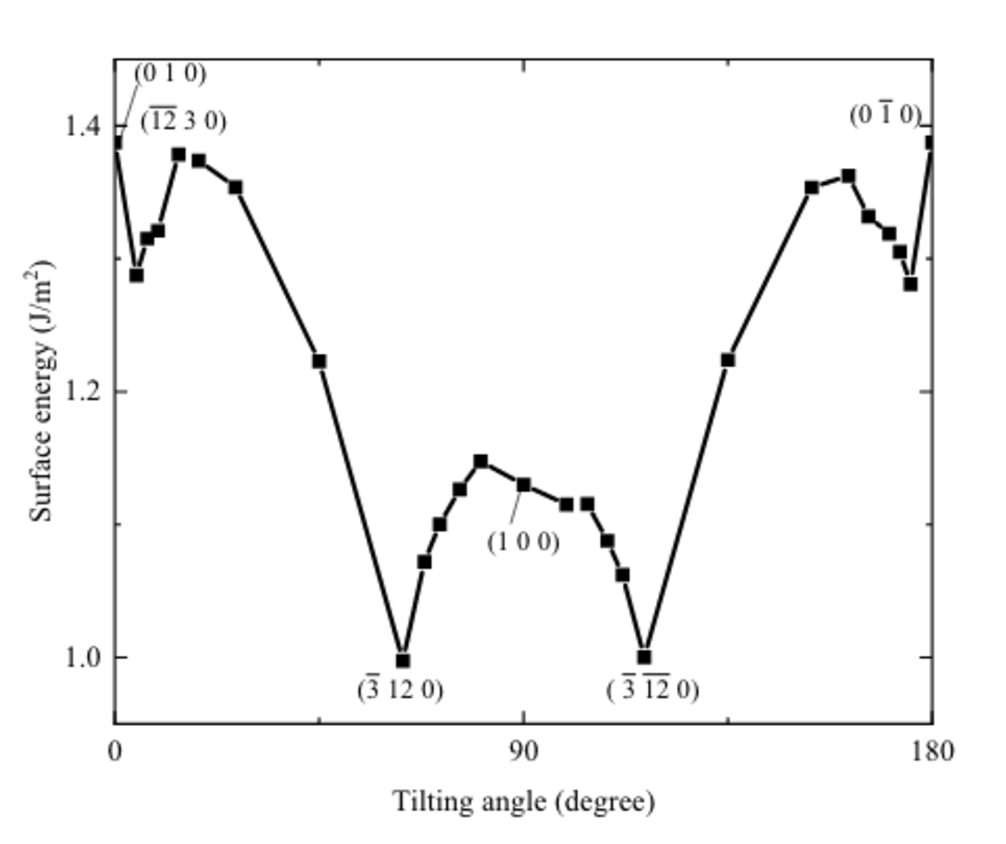
\includegraphics[width=\columnwidth]{fig2}
  \caption{The Surface Energy as a function of misorientation angle at 500 K.}
  \label{fig:2}
\end{figure}

\subsection{Work of Adhesion}

The work of adhesion (WAd) at 500 K is calculated via Equation \ref{eq:fform} and plotted as a function of the corresponding misorientation angle in Figure~\ref{fig:3}. The WAd is defined here as the energy required to form two surfaces from a given STGB. A lower value for the work of adhesion represents less total energy required to break apart a GB into two separate free surfaces. Thus, orientations with low WAd are potential sites for cleavage or fracture, or the nucleation of the $\alpha$ tearing phenomenon \cite{rest1993}. The maximum WAd is found for the (0 1 0) STGB and the minimum for the ($\overline{3}$ 15 0) STGB, with magnitudes of 2.4 J/m$^2$ and 1.43 J/m$^2$, respectively, as seen in Figure \ref{fig:3}. A simple average of the WAd yields a value of 1.78 J/m${^2}$. A possible twin in $\alpha$-U found from the current study is the ($\overline{3}$ 12 0)$\langle$1 0 0$\rangle$ STGB. Although this STGB is found to have a very low energy, its WAd value is not significantly higher or lower than the average WAd of the respective type of STGB. The WAd of this STGB is 1.76 J/m$^2$.

The $\alpha$-U WAd values can be compared with the available literature on the WAd of other fuel systems. At 300 K, the cleavage energy of UO$_\mathrm{2}$ \cite{emeric2019} GBs has a wide range, from 0.3 J/m$^2$ to 2.5 J/m$^2$ (maximum of 4.5 J/m$^2$ in Reference \cite{williams2015}). The work presented here demonstrates an approximate average WAd of 1.78 J/m$^2$ at 500 K, suggesting that the WAd of $\alpha$-U STGBs is likely to be within the upper range of UO$_\mathrm{2}$. $\alpha$-U has a lower average WAd than $\gamma$-U at 600 K (approximately 1.9 J/m$^2$) and U$_\mathrm{3}$Si$_\mathrm{2}$ (approximately 2.6 J/m$^2$) \cite{beeler2018,beeler2019}. Hence, $\alpha$-U is more prone to failure along GBs compared to other metallic uranium-based nuclear fuels.

\begin{figure}[ht] % replace 't' with 'b' to force it to be on the bottom
  \centering
  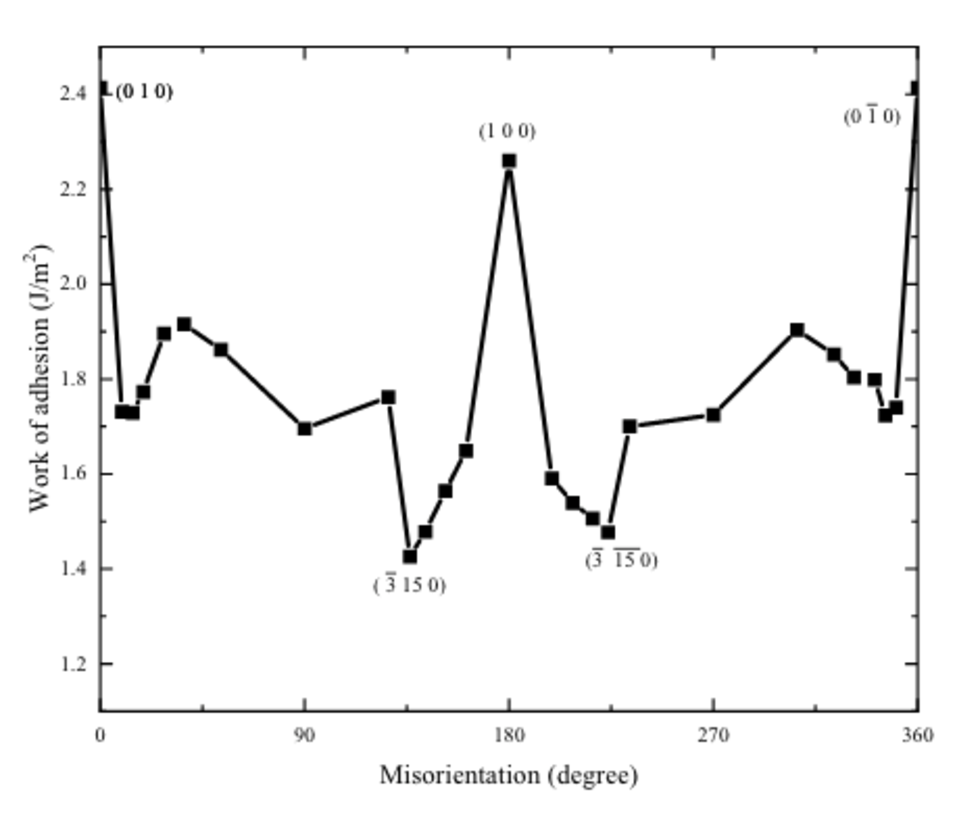
\includegraphics[width=\columnwidth]{fig3}
  \caption{The Work of Adhesion as a function of misorientation angle at 500 K.}
  \label{fig:3}
\end{figure}
%%%%%%%%%%%%%%%%%%%%%%%%%%%%%%%%%%%%%%%%

\subsection{Defect Interaction with Grain Boundaries}

Three unique grain boundaries are investigated to obtain the nature of defect interactions with grain boundaries in $\alpha$-U. In all three systems (denoted A, B, and C) an interstitial is utilized as the defect of interest, however a vacancy is only implemented in the first grain boundary type. The defect formation energy as a function of normalized distance is shown in Fig. \ref{fig:4}. The grain boundary is located at a normalized length of zero and the grain center is located at a normalized length of 0.5. The distance axis is noted as a normalized distance because each individual grain boundary is of a different total length. Defects in the center of the grain behave as if they resided in the bulk, and exhibit defect formation energies of those in bulk $\alpha$-U. Near the grain boundary defect formation energy changes, dependent upon both the defect type and the grain boundary type. For the grain boundary A, both interstitials and vacancies are attracted to the grain boundary, as evidenced by the reduction in formation energy as their distance from the grain boundary is reduced. The interstitial formation energy is reduced from approximately 2.8 eV to 0.2 eV, and the vacancy formation energy is reduced from 1.9 eV to 0.5 eV. These are both significant reductions in the defect formation energy and point towards strong interactions of grain boundaries with defects. The interaction distance is defined here as the distance from the grain boundary at which the formation energy is at an average of the bulk and grain boundary values. The interaction distance varies between interstitials and vacancies, with the interstitial observing the grain boundary at a significantly larger distance than the vacancy. For the A interstitial, the interaction distance is approximately 14 \AA. However, not all grain boundaries attract interstitials in the same manner, which is shown by comparing the B and C grain boundaries in Fig. \ref{fig:4}. These two grain boundaries show very little affinity for interstitials, and the reduction in the formation energy is less than 20\%. Additionally, the interaction distance is significantly reduced. 

While there are differences in the grain boundary energy and work of adhesion between three grain boundaries, trends can not be drawn from such a small sample size. As such, this work is being expanded in order to elucidate the effect of grain boundary orientation and energy on defect properties. 

\begin{figure}[ht] % replace 't' with 'b' to force it to be on the bottom
  \centering
  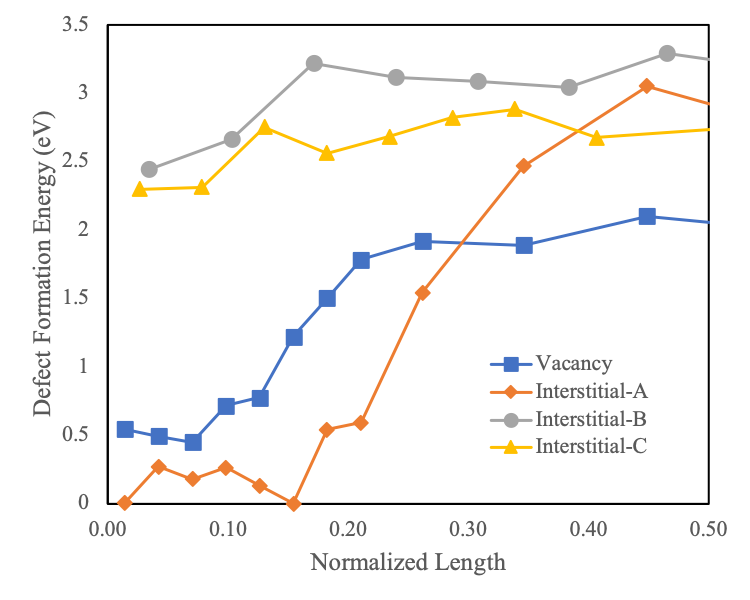
\includegraphics[width=\columnwidth]{fig4.png}
  \caption{The defect formation energy as a function of normalized length from a grain boundary for interstitials and a vacancy. Unique grain boundaries are denoted A, B, and C.}
  \label{fig:4}
\end{figure}

\FloatBarrier

%%%%%%%%%%%%%%%%%%%%%%%%%%%%%%%%%%%%%%%%%%%%%%%%%%%%%%%%%%%%%%%%%%%%%%%%%%%%%%%%
\section{Conclusions}

In this study, the grain boundary energy, surface energy, and work of adhesion of symmetric tilt grain boundaries in $\alpha$-U have been calculated as a function of misorientation angle. Twenty-four unique grain boundaries have been examined at 500 K to analyze the various interfacial properties. The lowest grain boundary energy is found at the ($\overline{3}$ $\overline{12}$ 0)$\langle$1 0 0$\rangle$ STGB, and has the potential to form twins. The lowest work of adhesion is found for the ($\overline{3}$ 12} 0)$\langle$1 0 0$\rangle$ STGB, which is the most likely cleavage surface investigated in this work. The arithmetic average of the surface energy (1.25 J/m$^2$) is approximately 1.5 times the GB energy (0.71 J/m$^2$), and the WAd is approximately twice the GB energy (1.78 J/m$^2$). Defect interactions with grain boundaries were studied, showing that both vacancies and interstitials can be attracted to grain boundaries and that the magnitude of the interaction varies dramatically depending upon the individual grain boundary of interest. Additionally, the interaction distance seems to correspond with the magnitude of the interaction of the defect with the grain boundary. The information from this work will be utilized to study grain boundary evolution in polycrystalline $\alpha$-U and deformation under irradiation.


%%%%%%%%%%%%%%%%%%%%%%%%%%%%%%%%%%%%%%%%%%%%%%%%%%%%%%%%%%%%%%%%%%%%%%%%%%%%%%%%
\section{Acknowledgments}
Work was supported through the INL Laboratory Directed Research and Development (LDRD) Program under DOE Idaho Operations Office Contract DE-AC07-05ID14517. This manuscript has been authored by Battelle Energy Alliance, LLC with the U.S. Department of Energy. The publisher, by accepting the article for publication, acknowledges that the U.S. Government retains a nonexclusive, paid-up, irrevocable, worldwide license to publish or reproduce the published form of this manuscript, or allow others to do so, for U.S. Government purposes. This research made use of the resources of the High-Performance Computing Center at Idaho National Laboratory, which is supported by the Office of Nuclear Energy of the U.S. Department of Energy and the Nuclear Science User Facilities.

%%%%%%%%%%%%%%%%%%%%%%%%%%%%%%%%%%%%%%%%%%%%%%%%%%%%%%%%%%%%%%%%%%%%%%%%%%%%%%%%
\bibliographystyle{ans}
\bibliography{../beelerbib}
\end{document}

